%%%%%%%%%%%%%%%%%%%%% chapter.tex %%%%%%%%%%%%%%%%%%%%%%%%%%%%%%%%%
%
% esempio di capitolo
%
% Usare questo  file come template per il vostro documento.
%
%%%%%%%%%%%%%%%%%%%%%%%% Springer-Verlag %%%%%%%%%%%%%%%%%%%%%%%%%%

\chapter{Titolo del capitolo}
\label{intro} % Fornire sempre un'unica label
% usare \chaptermark{}
% per alterare o aggiustare l'intestazione del capitolo nella running head

Il vostro testo va qui.  Suddividere il testo in paragrafi  con i comandi 
 standard di \LaTeX\ .

\section{Titolo di primo livello}
\label{sec:1}
% Fornire sempre un'unica label
% ed usare \ref{<label>} per i riferimenti (cross-references)
% e \cite{<label>} per le citazioni bibliografiche
% usare \sectionmark{}
% per alterare o aggiustare l'intestazione della sezione nella  running head
Il vostro testo va qui. Usare  i comandi standard di  \LaTeX\ per le citazioni e i riferimenti bibliografici
\cite{monograph}.

\subsection{Titolo di secondo livello}
\label{sec:2}
Il vostro testo va qui.

\begin{equation}
\vec{a}\times\vec{b}=\vec{c}
\end{equation}

\subsubsection{Titolo di terzo livello}
Il vostro testo va qui. % Usare l'automatismo \LaTeX\ per i riferimenti e per le citazioni, si veda la Sez.~\ref{sec:1}.

\paragraph{Titolo del paragrafo} %
Il vostro testo va qui.

\subparagraph{Titolo del sotto-paragrafo.} Il vostro testo va qui.%
%
\index{paragrafo}
% Usare il comando \index{} per inserire le proprie parole chiave
%
% Per le tabelle usare
%
\begin{table}
\centering
\caption{Scrivere qui la didascalia della tabella}
\label{tab:1}       % Fornire una label unica
%
% Per le tabelle LaTeX usare
%
\begin{tabular}{lll}
\hline\noalign{\smallskip}
prima & seconda & terza  \\
\noalign{\smallskip}\hline\noalign{\smallskip}
numero & numero & numero \\
numero & numero & numero \\
\noalign{\smallskip}\hline
\end{tabular}
\end{table}
%
%
% Per le figure usare
%
\begin{figure}
\centering
% Usare il comando appropriato per il vostro programma di inserzione dell figure
% per inserire il file immagine.
% Ad esempio, con l'opzione graphics usare
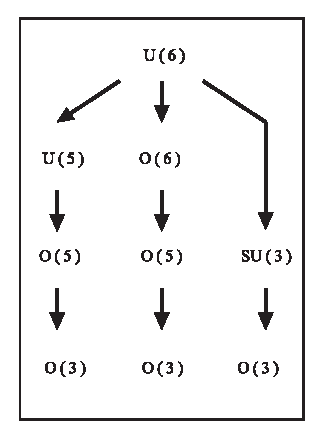
\includegraphics[height=4cm]{figure.eps}
%
% Altrimenti, usare
%\picplace{5cm}{2cm} % Fornire la corretta altezza e larghezza in cm
%
\caption{Scrivere qui la didascalia della figura}
\label{fig:1}       % Fornire una label unica
\end{figure}
%
% Per environments integrati usare
%
\begin{theorem}
Qui il testo del teorema.
\end{theorem}
%
% oppure
%
\begin{lemma}
Qui il testo del lemma.
\end{lemma}
%
%
% Problemi o Esercizi dovrebbero essere ordinati per capitolo
\section*{Problemi}
\addcontentsline{toc}{section}{Problemi}
%
% Use the following environment.
% Don't forget to label each problem;
% the label is needed for the solutions' environment
\begin{prob}
\label{prob1}
Il problema\footnote{Nota a pi\`{e} pagina} \`{e} descritto qui. Il problema \`{e} descritto qui. Il problema \`{e} descritto qui. \end{prob}

\begin{prob}
\label{prob2}
\textbf{Titolo del problema}\\
(a) La prima parte del problema \`{e} descritta qui.\\
(b) La seconda parte del problema \`{e} descritta qui.
\end{prob}



%
